\section{Resultados y discusión}

\subsection{Medición con multímetro}

La siguiente tabla muestra los resultados para las tres mediciones a distinta temperatura.
\begin{table}[H]
    \centering
    \footnotesize
    \caption{Resistencia y temperatura del termistor}
    \begin{tabular}{lccccccc}
    \toprule
    & Condición & Temperatura [°C] & Resistencia [$ k\Omega$] \\
    \midrule
        & Ambiente & 24 & 5.74  \\
        & Bajas temperaturas & 3 & 12.44  \\
        & Altas temperaturas & 76 & 1.27 \\
    \bottomrule
    \end{tabular}
    \end{table}
    \vspace{-0.5cm}
    Se observa en la tercera columna de la tabla que los resultados coinciden con lo esperado. Dado que el termistor utilizado tiene un coeficiente negativo, a mayores temperaturas su valor resistivo debería disminuir y, a menores temperaturas, aumentar.
    Al pasar de 24 °C a 3 °C (descenso), su resistencia aumentó $ 6.7  k\Omega$. Adicionalmente, al pasar de 24 °C a 76 °C (aumento), ésta disminuyó en $ 4.47  k\Omega$.
    
    Una principal fuente de error fue la medición de la temperatura ambiente, la cual fue de 24 °C cuando debería haber rondado los 19 °C. Consideramos que esto podría deberse a que se sostuvo el termopar con la mano, transfiriéndole calor a los cables de conexión y aumentando así la temperatura registrada. A su vez, la conexión con 
    el tester era inestable, ya que había que ubicarlo las terminales estuvieran en contacto y pudiera medir. Incluso, moviendo el dispositivo el registro variaba provocando grandes incertezas. Por otro lado,
    la variación de la resistencia del termistor respecto a la termperatura era tan rápida que el display del tester se encontraba constantemente en cambio en las tres pruebas. Por lo cual, para el caso de temperaturas altas, se tomó el mínimo valor alcanzado antes de que 
    volviera a subir; y en el caso de bajas temperaturas, el máximo valor antes de que comenzara a bajar. Finalmente, otra fuente de error podría haber sido que, al efectuar las mediciones con las terminales metálicas del termistor enrrolladas con las puntas del multímetro, cuando se introducían en los vasos con agua, ocurría un 
    leve cortocircuito a través del fluido, y no se registraba correctamente la resistencia del termistor. Por lo tanto, se sacaba un corto tiempo del agua lo cual también afectaba simultáneamente la temperatura a la cual se encontraba.


\subsection{Medición con arduino}
\underline{Coeficientes del fabricante}

La siguiente tabla expresa los valores de resistencia y temperatura del termistor registrados con el arduino empleando los coeficientes provistos por el fabricante
\begin{table}[H]
    \centering
    \footnotesize
    \caption{Resistencia y temperatura del termistor con coeficientes del fabricante}
    \begin{tabular}{lccccccc}
    \toprule
    & Condición & Temperatura [°C] & Resistencia [$ k\Omega$] \\
    \midrule
        & Ambiente & 23.1 & 11.40  \\
        & Bajas temperaturas & 3.8 & 28.32  \\
        & Altas temperaturas & 73.0 & 1.60 \\
    \bottomrule
    \end{tabular}
    \end{table}
    \vspace{-0.5cm}
Al efectuar las mismas mediciones con el circuito de Arduino, los valores de las temperaturas (2da columna) coindicen ampliamente con los detectados por el termopar; mientras que 
las resistencias matuvieron la relación inversamente proporcional entre resistividad y temperatura; pese a que las de condición ambiente y altas temperaturas difieren notablemente con las anteriores.

Una fuente de error fue la forma de conexión del termistor. Se usó como base un protoboard pero, como se debía colocar el termistor en los vasos con hielo y agua caliente, se optó por
emplear cables jumpers tipo macho-hembra, introduciendo las conexiones metálicas del dispositivo con la terminal macho para tener la extensión suficiente. Sin embargo,
la condición de la conexión era extremadamente inestable, incluso saliéndose y teniendo que reconectarlos; por lo cual este contacto deficiente pudo haber influido en las mediciones. Por otro lado, hay un delay entre que se detectan los valores en el termistor, se
convierten a valores digitales y se muestran en pantalla, por lo que los registros estaban constantemente cambiando y se tomaron los valores que más cercanos estaban entre sí y con mayor frecuencia. 

\underline{Coeficientes calculados}

Con la página web mencionada en la sección 3.2, se obtuvieron los siguientes coeficientes de la ecuación de Steinhart - Hart: A = 0.020457197768074423; B = -0.003374640051255977; C = 0.000017874326825975414

\begin{table}[H]
    \centering
    \footnotesize
    \caption{Resistencia y temperatura del termistor con coeficientes calculados}
    \begin{tabular}{lccccccc}
    \toprule
    & Condición & Temperatura [°C] & Resistencia [$ k\Omega$] \\
    \midrule
        & Ambiente & 5 & 12.0  \\
        & Bajas temperaturas & -11 & 23.4 \\
        & Altas temperaturas & 51 & 2.5 \\
    \bottomrule
    \end{tabular}
    \end{table}
    \vspace{-0.5cm}
    En este caso, los valores de las resistencias son ampliamente similares a los obtenidos con los coeficientes del fabricante. Sin embargo, las temperaturas son 
    extremadamente distintas, incluso incoherentes ya que la del vaso con hielo alcanzó valores muy negativos; la de temperatura ambiente mucho menor a la del momento y la caliente mucho más chica
    a la registrada previamente. Además, se midió con el termopar en ese momento la del vaso con agua caliente para analizar si en el tiempo transcurrido podría haber bajado tanto la temperatura, pero éste
    devolvió en el display del multímetro 72 °C.
    
    Si bien las fuentes de error explicadas anteriormente también aplican para este caso, la principal aquí se debe a los coeficientes calculados en el programa. Por un lado, estos requieren de la temperatura expresada en F, 
    la cual fue redondeada para simplicidad de los cálculos; además de que empleó los 24 °C para la temperatura ambiente que, como se aclaró previamente, no era fiable. Por otro lado, los coeficientes son del orden de $10^{-3}$ y $10^{-5}$, es decir, muy pequeños y, 
    además, se encuentran en el denominador de la ecuación de Steinhart - Hart, por lo que pequeñas perturbaciones en los mismos hacen que los resultados difieran considerablemente. Consideramos que esta es la principal fuente de error para los cálculos de la temperatura.

\subsection{Curvas características}
\begin{figure}[htbp]
\centering
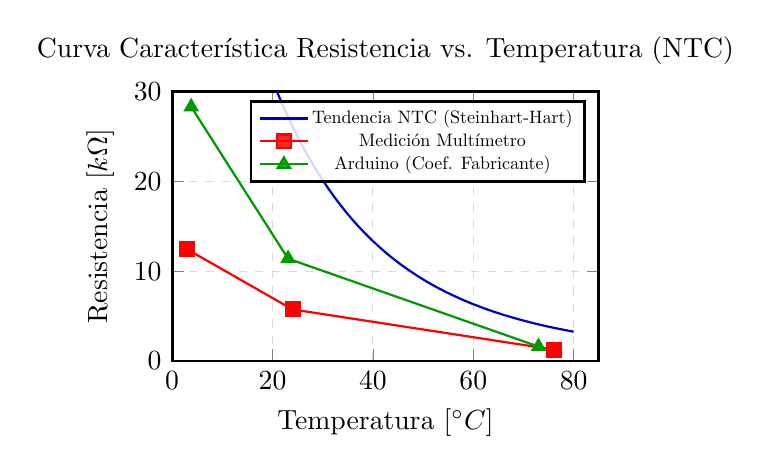
\begin{tikzpicture}
\begin{axis}[
    width=7cm,
    height=5cm,
    title={Curva Característica Resistencia vs. Temperatura (NTC)},
    xlabel={Temperatura [$^\circ\text{C}$]},
    ylabel={Resistencia [$\text{k}\Omega$]},
    xmin=0, xmax=85,
    ymin=0, ymax=30,
    grid=both,
    grid style={dashed, gray!30},
    legend pos=north east,
    legend style={
        nodes={scale=0.65, transform shape},
        fill=white,
        fill opacity=0.85,
        text opacity=1
    },
    line width=1pt
]

% Curva 1: Modelo Teórico Steinhart-Hart
\addplot[
    domain=2:80, 
    samples=100, 
    color=blue!80!black,
    thick
] 
{25 * exp(3900*(1/(x+273.15) - 1/298.15))};
\addlegendentry{Tendencia NTC (Steinhart-Hart)}

% Curva 2: Medición con Multímetro (puntos unidos por líneas)[cite: 1]
\addplot[
    color=red,
    mark=square*,
    mark size=2.5pt,
    thick
]
coordinates {
    (3, 12.44)
    (24, 5.74)
    (76, 1.27)
};
\addlegendentry{Medición Multímetro}

% Curva 3: Arduino Coeficientes del Fabricante (puntos unidos por líneas)[cite: 1]
\addplot[
    color=green!60!black,
    mark=triangle*,
    mark size=2.5pt,
    thick
]
coordinates {
    (3.8, 28.32)
    (23.1, 11.40)
    (73.0, 1.60)
};
\addlegendentry{Arduino (Coef. Fabricante)}

\end{axis}
\end{tikzpicture}
\caption{Relación inversamente proporcional entre la resistencia eléctrica y la temperatura del termistor NTC analizado en laboratorio.}
\label{fig:curva_ntc}
\end{figure}

El comportamiento electrotérmico del sensor NTC representado en la figura 2 permite corroborar de manera empírica la naturaleza no lineal del dispositivo semiconductor. La curva continua de tendencia teórica, modelada mediante la relación exponencial de Steinhart-Hart, establece el perfil ideal de transferencia donde la resistencia alcanza sus valores más elevados a temperaturas bajas y decrece de forma pronunciada a medida que la temperatura aumenta, asintotizándose en el rango térmico superior. Las dos trayectorias experimentales trazadas a partir de las mediciones del multímetro y del módulo Arduino con los coeficientes del fabricante acompañan cualitativamente esta misma dinámica decreciente, confirmando la validez del coeficiente de temperatura negativo del componente.

Al analizar la curva correspondiente a las mediciones directas con multímetro, se observa que los valores resistivos registrados ($12.44\,\text{k}\Omega$ a $3^{\circ}\text{C}$, $5.74\,\text{k}\Omega$ a $24^{\circ}\text{C}$ y $1.27\,\text{k}\Omega$ a $76^{\circ}\text{C}$) mantienen una pendiente suave y coherente con el perfil esperado. Sin embargo, la desviación cuantitativa observada respecto a la curva teórica y a la adquisición por microprocesador responde directamente a las incertidumbres introducidas por el método manual. La falta de un acoplamiento mecánico firme entre las puntas de prueba y los terminales del termistor generó variaciones en la resistencia de contacto. A su vez, la rápida respuesta del material ante el intercambio térmico con los fluidos hizo que la lectura en la pantalla digital del óhmetro no alcanzara un régimen estacionario definitivo, obligando a tomar los valores máximos y mínimos instantáneos justo antes del retorno térmico.

Por otro lado, la curva obtenida mediante la placa Arduino UNO con los coeficientes del fabricante registra valores de resistencia notablemente superiores en la región de bajas temperaturas ($28.32\,\text{k}\Omega$ a $3.8^{\circ}\text{C}$ y $11.40\,\text{k}\Omega$ a $23.1^{\circ}\text{C}$). Esta discrepancia respecto a las lecturas del multímetro se fundamenta en las diferencias metodológicas de acondicionamiento y adquisición de señal. La configuración del circuito divisor de tensión conectado a la entrada analógica del microcontrolador somete al circuito a un proceso de conversión analógico-digital (ADC) que promedia internamente las lecturas en presencia de retardo dinámico (\textit{delay}). Asimismo, la presencia de conexiones inestables mediante cables tipo \textit{jumper} en el protoboard y la influencia de ruido térmico y eléctrico no filtrado en la entrada del conversor alteraron la magnitud resistiva calculada por el programa, aunque manteniendo la precisión en la reconstrucción final de la temperatura ($3.8^{\circ}\text{C}$, $23.1^{\circ}\text{C}$ y $73.0^{\circ}\text{C}$) gracias a la robustez intrínseca de los coeficientes de calibración originales del fabricante.